\def\chapdir{./Chapter05}

\chapter{Database Layer} \label{ch:database-layer}

\section{Database Architecture}

\subsection{Overall Database Design Philosophy}

The OllamaNet platform employs a robust database architecture that balances the needs of a microservices ecosystem with the benefits of relational data integrity. The database layer is designed around several key principles:

\begin{enumerate}
   \item \textbf{Shared Database with Logical Separation}: While microservices often employ separate databases, OllamaNet uses a shared SQL Server database with logical separation to maintain data integrity while providing service isolation.

   \item \textbf{Repository Pattern}: Data access is abstracted through repositories, providing a consistent interface for services to interact with the database.

   \item \textbf{Unit of Work Pattern}: Transactions across multiple repositories are coordinated through a Unit of Work implementation, ensuring data consistency.

   \item \textbf{Domain-Driven Design}: The database schema reflects the domain model, with clear entity boundaries and relationships that map to business concepts.

   \item \textbf{Soft Delete}: Entities implement soft deletion to preserve historical data while allowing logical removal.
\end{enumerate}

\begin{figure}[p]
    \centering
    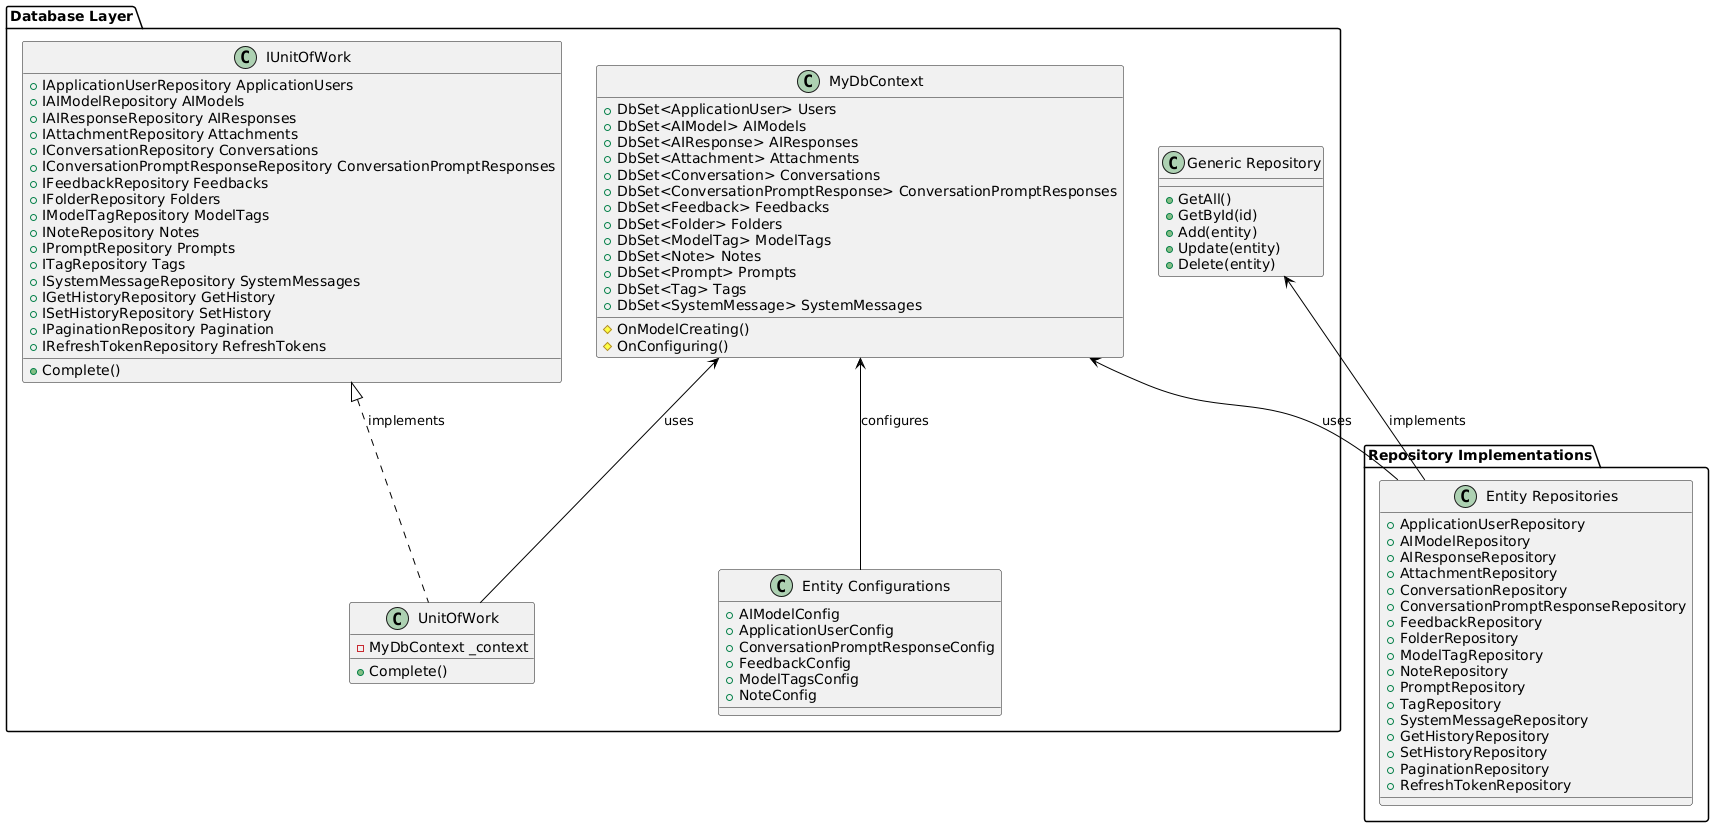
\includegraphics[width=\textwidth]{./Chapter05/figures/database_architecture.png}
    \caption{Database Architecture Overview}
    \label{fig:database-architecture}
\end{figure}
\clearpage

\subsection{Database Per Service Pattern Consideration}

The OllamaNet architecture considered the Database-per-Service pattern, which is common in microservices architectures, but ultimately chose a shared database approach for several reasons:

\begin{enumerate}
   \item \textbf{Data Integrity}: A shared database ensures referential integrity across services, which is particularly important for user data and relationships.

   \item \textbf{Simplified Deployment}: A single database reduces operational complexity compared to managing multiple databases.

   \item \textbf{Query Efficiency}: Cross-service queries can be performed more efficiently within a single database.

   \item \textbf{Transaction Support}: ACID transactions across related data are easier to implement in a shared database.
\end{enumerate}

However, to maintain service independence, the architecture implements logical separation through:

\begin{enumerate}
   \item \textbf{Service-Specific Repositories}: Each service accesses only its relevant entities through dedicated repositories.

   \item \textbf{Schema Namespacing}: Database tables are organized into logical groups aligned with service boundaries.

   \item \textbf{Access Control}: Services are restricted to their own data domains through repository interfaces.
\end{enumerate}

\subsection{Shared Database Implementation}

The shared database implementation uses Entity Framework Core as an ORM, with the following components:

\begin{enumerate}
   \item \textbf{Central DbContext}: A single \texttt{MyDbContext} class that extends \texttt{IdentityDbContext<ApplicationUser>} and includes all entity DbSets.

   \item \textbf{Entity Configuration}: Entity relationships and constraints are configured in the \texttt{OnModelCreating} method of the DbContext.

   \item \textbf{Service-Specific Repositories}: Each service has dedicated repositories that access only the entities relevant to that service.

   \item \textbf{Unit of Work Coordinator}: A central \texttt{UnitOfWork} class coordinates operations across repositories and manages transactions.
\end{enumerate}

\begin{verbatim}
public class MyDbContext : IdentityDbContext<ApplicationUser>
{
    public MyDbContext(DbContextOptions<MyDbContext> options) : base(options) { }

    public DbSet<AIModel> AIModels { get; set; }
    public DbSet<AIResponse> AIResponses { get; set; }
    public DbSet<Attachment> Attachments { get; set; }
    public DbSet<Conversation> Conversations { get; set; }
    public DbSet<ConversationPromptResponse> ConversationPromptResponses { get; set; }
    public DbSet<Feedback> Feedbacks { get; set; }
    public DbSet<ModelTag> ModelTags { get; set; }
    public DbSet<Prompt> Prompts { get; set; }
    public DbSet<RefreshToken> RefreshTokens { get; set; }
    public DbSet<SystemMessage> SystemMessages { get; set; }
    public DbSet<Tag> Tags { get; set; }

    protected override void OnModelCreating(ModelBuilder modelBuilder)
    {
        base.OnModelCreating(modelBuilder);

        // Configure ModelTag as a join entity
        modelBuilder.Entity<ModelTag>().HasKey(mt => new { mt.ModelId, mt.TagId });

        // Other entity configurations...
    }
}
\end{verbatim}

\subsection{Physical vs. Logical Database Separation}

OllamaNet employs logical separation within a physically shared database:

\begin{enumerate}
   \item \textbf{Physical Sharing}: All services access the same SQL Server instance and database.

   \item \textbf{Logical Separation}:
   \begin{itemize}
      \item Each service accesses only its domain-specific entities
      \item Repository interfaces expose only relevant operations
      \item Service boundaries are enforced at the application level
   \end{itemize}
\end{enumerate}

This approach provides several benefits:

\begin{itemize}
   \item \textbf{Data Consistency}: Ensures consistent data across services.
   \item \textbf{Simplified Transactions}: Enables ACID transactions across related entities.
   \item \textbf{Efficient Queries}: Allows for efficient joins between related entities.
   \item \textbf{Reduced Operational Complexity}: Simplifies database management and deployment.
\end{itemize}

\begin{figure}[p]
    \centering
    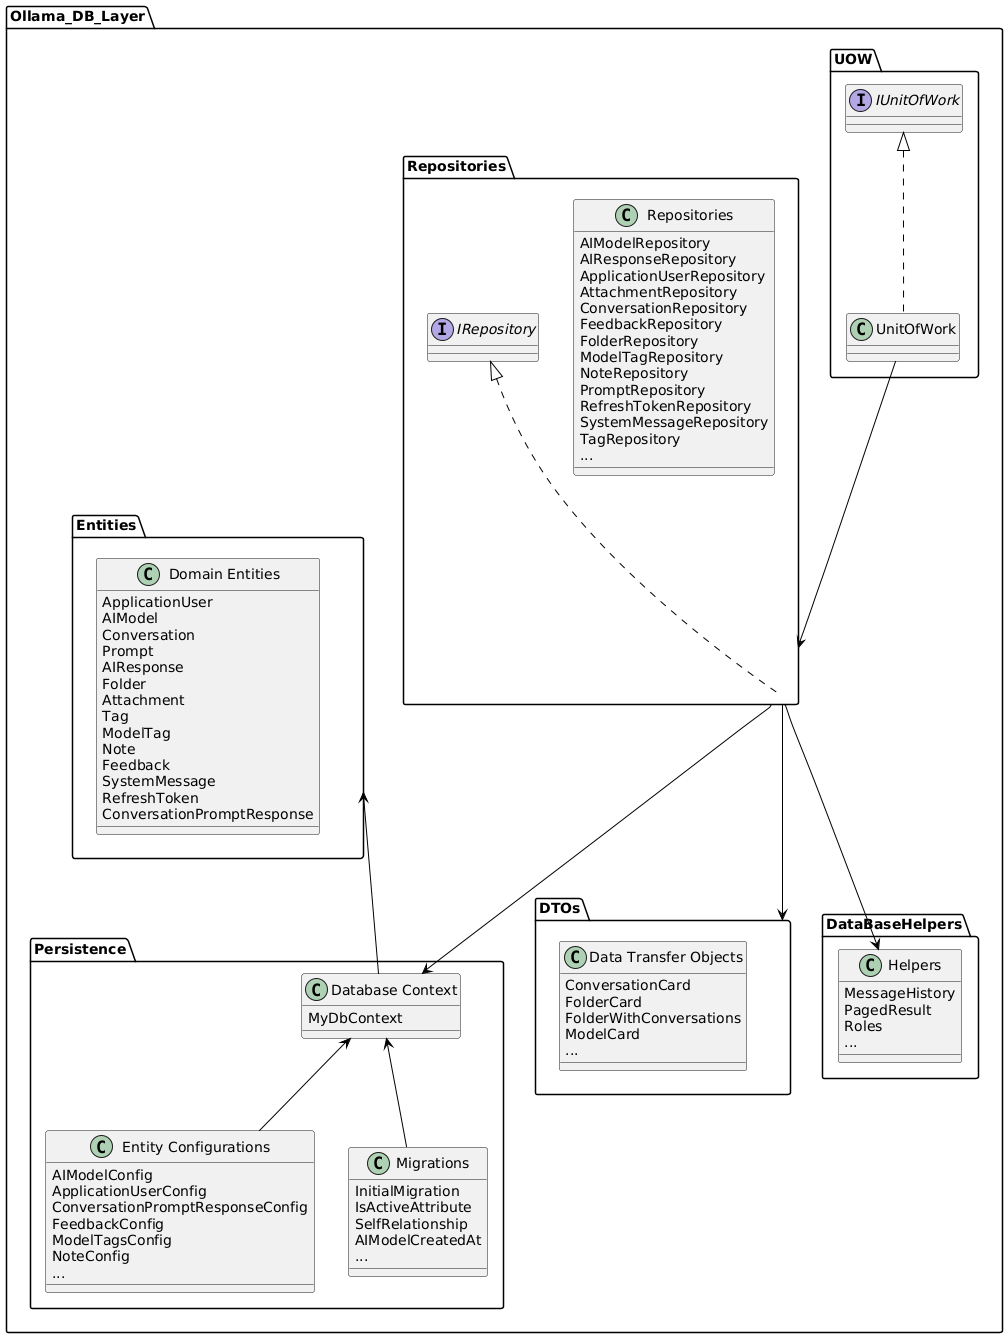
\includegraphics[width=\textwidth]{./Chapter05/figures/logical_separation.png}
    \caption{Physical vs Logical Database Separation}
    \label{fig:logical-separation}
\end{figure}
\clearpage

\subsection{Design Principles and Patterns}

The database layer implements several key design principles and patterns:

\subsubsection*{Repository Pattern}

Abstracts data access logic and provides a consistent interface for working with entities.

\begin{verbatim}
public interface IRepository<T> where T : class
{
    Task<IEnumerable<T>> GetAllAsync();
    Task<T> GetByIdAsync(string id);
    Task<bool> AddAsync(T entity);
    Task<bool> UpdateAsync(T entity);
    Task<bool> DeleteAsync(string id);
    Task<bool> SoftDeleteAsync(string id);
    Task<bool> ExistsAsync(string id);
}
\end{verbatim}

\subsubsection*{Unit of Work Pattern}

Coordinates operations across multiple repositories and provides a single point for committing changes.

\begin{verbatim}
public interface IUnitOfWork : IDisposable
{
    IAIModelRepository AIModels { get; }
    IAIResponseRepository AIResponses { get; }
    // Other repositories...
    
    Task<int> SaveChangesAsync();
}
\end{verbatim}

\subsubsection*{Identity Integration}

Extends ASP.NET Identity with custom user properties and relationships.

\subsubsection*{Soft Delete Pattern}

Implements logical deletion through an \texttt{IsDeleted} flag on entities.

\subsubsection*{Query Specification Pattern}

Encapsulates query logic for complex filtering and sorting.

\subsubsection*{Eager Loading Strategy}

Uses explicit loading of related entities to avoid N+1 query problems.

\section{Data Models}

\subsection{Entity Relationship Diagrams}

The OllamaNet database schema includes several interconnected entities that support the platform's functionality:

\begin{figure}[p]
    \centering
    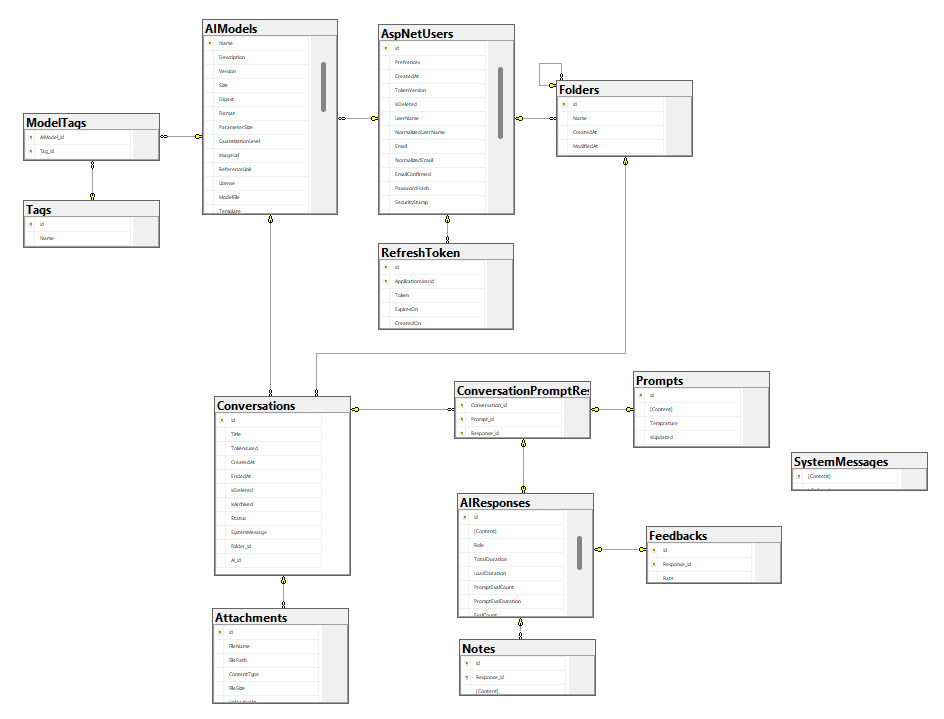
\includegraphics[width=\textwidth]{./Chapter05/figures/entity_relationship.png}
    \caption{Entity Relationship Diagram}
    \label{fig:entity-relationship}
\end{figure}
\clearpage

\subsection{Schema Designs}

The database schema is organized around several key domains:

\begin{enumerate}
   \item \textbf{User Management Domain}:
   \begin{itemize}
      \item ApplicationUser (extends IdentityUser)
      \item RefreshToken
   \end{itemize}

   \item \textbf{Model Management Domain}:
   \begin{itemize}
      \item AIModel
      \item Tag
      \item ModelTag (junction entity)
   \end{itemize}

   \item \textbf{Conversation Domain}:
   \begin{itemize}
      \item Conversation
      \item ConversationPromptResponse
      \item Prompt
      \item AIResponse
      \item Attachment
      \item Feedback
   \end{itemize}

   \item \textbf{System Configuration Domain}:
   \begin{itemize}
      \item SystemMessage
   \end{itemize}
\end{enumerate}

Each entity includes standard fields for tracking creation, modification, and deletion:

\begin{verbatim}
// Common fields found in most entities
public string Id { get; set; }
public DateTime CreatedAt { get; set; }
public bool IsDeleted { get; set; }
\end{verbatim}

\subsection{Domain Model to Database Mapping}

The OllamaNet platform maps its domain model to the database schema using Entity Framework Core's fluent API and data annotations:

\begin{enumerate}
   \item \textbf{Entity Configuration}:
   \begin{itemize}
      \item Primary keys defined using the \texttt{[Key]} attribute or fluent API
      \item Foreign keys established through the fluent API
      \item Navigation properties configured for relationships
   \end{itemize}

   \item \textbf{Relationship Mapping}:
   \begin{itemize}
      \item One-to-Many: Defined through navigation properties and foreign keys
      \item Many-to-Many: Implemented using junction entities (e.g., ModelTag)
      \item One-to-One: Configured with unique foreign keys
   \end{itemize}

   \item \textbf{Property Mapping}:
   \begin{itemize}
      \item Data types specified through attributes or fluent API
      \item Required fields marked with the \texttt{[Required]} attribute
      \item String length constraints applied where appropriate
   \end{itemize}
\end{enumerate}

Example of entity configuration in the DbContext:

\begin{verbatim}
protected override void OnModelCreating(ModelBuilder modelBuilder)
{
    base.OnModelCreating(modelBuilder);

    // Configure ModelTag as a join entity
    modelBuilder.Entity<ModelTag>().HasKey(mt => new { mt.ModelId, mt.TagId });

    modelBuilder.Entity<ModelTag>()
        .HasOne(mt => mt.Model)
        .WithMany(m => m.ModelTags)
        .HasForeignKey(mt => mt.ModelId);

    modelBuilder.Entity<ModelTag>()
        .HasOne(mt => mt.Tag)
        .WithMany(t => t.ModelTags)
        .HasForeignKey(mt => mt.TagId);
}
\end{verbatim}

\subsection{Database Constraints and Validations}

The OllamaNet database implements several types of constraints and validations:

\begin{enumerate}
   \item \textbf{Primary Key Constraints}: Each entity has a unique identifier, typically a string containing a GUID.

   \item \textbf{Foreign Key Constraints}: Relationships between entities are enforced through foreign keys.

   \item \textbf{Required Field Constraints}: Critical fields are marked as required to prevent null values.

   \item \textbf{String Length Constraints}: String fields have appropriate length constraints.

   \item \textbf{Unique Constraints}: Applied to fields that must be unique, such as usernames and email addresses.

   \item \textbf{Default Values}: Some fields have default values, such as \texttt{IsDeleted = false} and \texttt{CreatedAt = DateTime.UtcNow}.

   \item \textbf{Check Constraints}: Used to enforce business rules, such as valid status values.
\end{enumerate}

These constraints are implemented through a combination of Entity Framework Core configurations and database-level constraints.

\subsection{Soft Delete Implementation}

OllamaNet implements soft deletion across its entities to preserve historical data while allowing logical removal:

\begin{enumerate}
   \item \textbf{IsDeleted Flag}: Each entity includes an \texttt{IsDeleted} boolean property.

   \item \textbf{Repository Filtering}: Repositories automatically filter out entities where \texttt{IsDeleted = true}.

\begin{verbatim}
public async Task<IEnumerable<Tag>> GetAllAsync()
{
    return await _context.Tags
        .Where(t => !t.IsDeleted)
        .ToListAsync();
}
\end{verbatim}

   \item \textbf{Soft Delete Operation}: Instead of physically removing entities, the \texttt{SoftDeleteAsync} method sets \texttt{IsDeleted = true}.

\begin{verbatim}
public async Task<bool> SoftDeleteAsync(string id)
{
    var tag = await _context.Tags.FindAsync(id);
    if (tag == null)
        return false;

    tag.IsDeleted = true;
    _context.Tags.Update(tag);
    return true;
}
\end{verbatim}

   \item \textbf{Query Extensions}: Extension methods automatically apply soft delete filtering to queries.
\end{enumerate}

This approach provides several benefits:
\begin{itemize}
   \item Preserves historical data for auditing and analysis
   \item Allows for data recovery if needed
   \item Maintains referential integrity across related entities
   \item Simplifies compliance with data retention requirements
\end{itemize}

\section{Data Consistency Strategies}

\subsection{Eventual Consistency Approaches}

While OllamaNet primarily uses a shared database with strong consistency, it also implements eventual consistency patterns for specific scenarios:

\begin{enumerate}
   \item \textbf{Cache Synchronization}: Redis caching is used with appropriate invalidation strategies to ensure eventual consistency between the cache and the database.

   \item \textbf{Read-Your-Writes Consistency}: The system ensures that after a write operation, subsequent reads will reflect the changes, even when caching is involved.

   \item \textbf{Background Processing}: Some operations are performed asynchronously, with eventual consistency guaranteed through reliable message processing.

   \item \textbf{Optimistic Concurrency}: Entity Framework's optimistic concurrency control is used to detect and resolve conflicts when multiple services update the same data.
\end{enumerate}

\subsection{Saga Pattern Implementation}

For complex operations that span multiple services, OllamaNet implements a simplified version of the Saga pattern:

\begin{enumerate}
   \item \textbf{Coordinated Transactions}: The Unit of Work pattern coordinates transactions within a single service.

   \item \textbf{Compensating Transactions}: For cross-service operations, compensating transactions are implemented to roll back changes if a step fails.

   \item \textbf{Event-Driven Coordination}: Services publish events to signal completion of their part of a distributed transaction.
\end{enumerate}

This approach helps maintain data consistency across service boundaries while avoiding distributed transactions.

\subsection{Distributed Transactions Handling}

OllamaNet avoids distributed transactions where possible, but implements several strategies for maintaining consistency across services:

\begin{enumerate}
   \item \textbf{Service Composition}: Complex operations are composed at the API level rather than using distributed transactions.

   \item \textbf{Event-Driven Updates}: Services subscribe to events from other services to update their data accordingly.

   \item \textbf{Idempotent Operations}: APIs are designed to be idempotent, allowing safe retries of failed operations.

   \item \textbf{Consistency Verification}: Background processes verify and reconcile data consistency across services.
\end{enumerate}

\subsection{Concurrency Control Mechanisms}

The database layer implements several concurrency control mechanisms:

\begin{enumerate}
   \item \textbf{Optimistic Concurrency}: Entity Framework's optimistic concurrency control is used to detect conflicts during updates.

\begin{verbatim}
modelBuilder.Entity<AIModel>()
    .Property(p => p.RowVersion)
    .IsRowVersion();
\end{verbatim}

   \item \textbf{Pessimistic Locking}: For critical operations, explicit database locks are used to prevent concurrent modifications.

   \item \textbf{Transaction Isolation Levels}: Appropriate transaction isolation levels are set based on the operation's requirements.

\begin{verbatim}
using var transaction = await _context.Database.BeginTransactionAsync(IsolationLevel.ReadCommitted);
try
{
    // Perform operations
    await _context.SaveChangesAsync();
    await transaction.CommitAsync();
}
catch
{
    await transaction.RollbackAsync();
    throw;
}
\end{verbatim}
\end{enumerate}

\subsection{Error Handling and Rollback Strategies}

The database layer implements robust error handling and rollback strategies:

\begin{enumerate}
   \item \textbf{Transaction Scope}: Operations that modify multiple entities are wrapped in transactions to ensure atomicity.

\begin{verbatim}
public async Task<bool> CreateConversationWithPromptAsync(Conversation conversation, Prompt prompt, AIResponse response)
{
    // Add entities
    await _unitOfWork.Conversations.AddAsync(conversation);
    await _unitOfWork.Prompts.AddAsync(prompt);
    await _unitOfWork.AIResponses.AddAsync(response);
    
    // Create relationship
    var cpr = new ConversationPromptResponse
    {
        Id = Guid.NewGuid().ToString(),
        ConversationId = conversation.Id,
        PromptId = prompt.Id,
        AIResponseId = response.Id,
        CreatedAt = DateTime.UtcNow
    };
    
    await _unitOfWork.ConversationPromptResponses.AddAsync(cpr);
    
    // Save all changes in a single transaction
    await _unitOfWork.SaveChangesAsync();
    
    return true;
}
\end{verbatim}

   \item \textbf{Exception Handling}: Exceptions during database operations are caught and handled appropriately, with transactions rolled back when necessary.

   \item \textbf{Retry Logic}: Transient errors are handled with retry logic to improve resilience.

   \item \textbf{Logging}: Database errors are logged with sufficient context for troubleshooting.
\end{enumerate}

\section{Database Technologies}

\subsection{SQL Server Implementation Details}

OllamaNet uses SQL Server as its primary database technology:

\begin{enumerate}
   \item \textbf{Version}: SQL Server 2019 or later, supporting modern features like JSON support and improved performance.

   \item \textbf{Connection Management}: Connection pooling is configured for optimal performance and resource utilization.

   \item \textbf{Indexing Strategy}: Appropriate indexes are created for frequently queried fields to optimize performance.

   \item \textbf{Query Optimization}: Complex queries are optimized using query hints and execution plan analysis.

   \item \textbf{Security Configuration}: SQL Server is configured with appropriate security settings, including encryption and access controls.
\end{enumerate}

\subsection{Entity Framework Core Configuration}

Entity Framework Core is configured for optimal performance and functionality:

\begin{enumerate}
   \item \textbf{DbContext Configuration}: The \texttt{MyDbContext} is configured with appropriate options for tracking, batching, and logging.

\begin{verbatim}
services.AddDbContext<MyDbContext>(options =>
    options.UseSqlServer(Configuration.GetConnectionString("DefaultConnection"),
        sqlOptions =>
        {
            sqlOptions.EnableRetryOnFailure(
                maxRetryCount: 5,
                maxRetryDelay: TimeSpan.FromSeconds(30),
                errorNumbersToAdd: null);
        })
    .UseQueryTrackingBehavior(QueryTrackingBehavior.NoTracking)
    .EnableSensitiveDataLogging(isDevelopment));
\end{verbatim}

   \item \textbf{Entity Configuration}: Entities are configured using a combination of data annotations and the fluent API.

   \item \textbf{Lazy Loading}: Lazy loading is disabled by default to prevent N+1 query problems, with explicit loading used when needed.

   \item \textbf{Query Filters}: Global query filters are applied for soft delete and multi-tenancy.

\begin{verbatim}
modelBuilder.Entity<Conversation>()
    .HasQueryFilter(c => !c.IsDeleted);
\end{verbatim}

   \item \textbf{Performance Optimization}: Query compilation is cached, and query execution is optimized through appropriate includes and projections.
\end{enumerate}

\subsection{Redis Caching Implementation}

OllamaNet uses Redis for distributed caching to improve performance:

\begin{enumerate}
   \item \textbf{Cache Architecture}: A multi-level caching approach with in-memory and Redis caches.

   \item \textbf{Cache-Aside Pattern}: Data is retrieved from the cache first, with database fallback when needed.

\begin{verbatim}
public async Task<T> GetOrSetAsync<T>(string key, Func<Task<T>> factory, TimeSpan? expiry = null)
{
    try
    {
        var cachedValue = await _redisCacheService.GetAsync<T>(key);
        if (cachedValue != null)
        {
            _logger.LogDebug("Cache hit for key: {Key}", key);
            return cachedValue;
        }

        _logger.LogDebug("Cache miss for key: {Key}", key);
        var result = await factory();
        
        if (result != null)
        {
            await _redisCacheService.SetAsync(key, result, expiry ?? _defaultExpiry);
        }
        
        return result;
    }
    catch (Exception ex)
    {
        _logger.LogWarning(ex, "Cache operation failed for key: {Key}, falling back to data source", key);
        return await factory();
    }
}
\end{verbatim}

   \item \textbf{Cache Invalidation}: When data changes, related cache entries are invalidated to maintain consistency.

   \item \textbf{Cache Resilience}: The system gracefully handles Redis unavailability by falling back to the database.

   \item \textbf{Cache Optimization}: Frequently accessed data is cached with appropriate expiration policies.
\end{enumerate}

\subsection{Query Optimization Techniques}

OllamaNet implements several query optimization techniques:

\begin{enumerate}
   \item \textbf{Indexing Strategy}: Appropriate indexes are created for frequently queried fields.

   \item \textbf{Query Projection}: Queries project only the required fields rather than loading entire entities.

\begin{verbatim}
public async Task<IEnumerable<ModelDto>> GetAllModelsAsync()
{
    return await _context.AIModels
        .Where(m => !m.IsDeleted)
        .Select(m => new ModelDto
        {
            Id = m.Id,
            Name = m.Name,
            Description = m.Description,
            // Only select needed properties
        })
        .ToListAsync();
}
\end{verbatim}

   \item \textbf{Eager Loading}: Related entities are loaded using explicit includes to avoid N+1 query problems.

\begin{verbatim}
public async Task<Conversation> GetConversationWithDetailsAsync(string id)
{
    return await _context.Conversations
        .Include(c => c.ConversationPromptResponses)
            .ThenInclude(cpr => cpr.Prompt)
        .Include(c => c.ConversationPromptResponses)
            .ThenInclude(cpr => cpr.AIResponse)
        .FirstOrDefaultAsync(c => c.Id == id && !c.IsDeleted);
}
\end{verbatim}

   \item \textbf{Pagination}: Large result sets are paginated to improve performance.

\begin{verbatim}
public async Task<IEnumerable<Conversation>> GetConversationsPagedAsync(
    string userId, int pageNumber, int pageSize)
{
    return await _context.Conversations
        .Where(c => c.UserId == userId && !c.IsDeleted)
        .OrderByDescending(c => c.CreatedAt)
        .Skip((pageNumber - 1) * pageSize)
        .Take(pageSize)
        .ToListAsync();
}
\end{verbatim}

   \item \textbf{Query Caching}: Frequently executed queries are cached to reduce database load.
\end{enumerate}

\subsection{Connection Management}

OllamaNet implements effective connection management strategies:

\begin{enumerate}
   \item \textbf{Connection Pooling}: Entity Framework Core's connection pooling is configured for optimal performance.

   \item \textbf{Connection Resilience}: Retry logic is implemented for transient connection failures.

   \item \textbf{Connection Monitoring}: Connection usage is monitored to detect leaks and performance issues.

   \item \textbf{Connection Timeout}: Appropriate connection timeouts are configured to prevent resource exhaustion.

   \item \textbf{Connection Security}: Connections use encrypted communication and minimal privilege accounts.
\end{enumerate}

\section{Data Migration and Versioning}

\subsection{Migration Strategy}

OllamaNet uses Entity Framework Core migrations for database schema evolution:

\begin{enumerate}
   \item \textbf{Migration Generation}: Migrations are generated using the EF Core Tools when entity models change.

\begin{verbatim}
dotnet ef migrations add AddConversationStatus
\end{verbatim}

   \item \textbf{Migration Application}: Migrations are applied during application startup or through deployment scripts.

\begin{verbatim}
public void Configure(IApplicationBuilder app, IWebHostEnvironment env)
{
    // Apply migrations at startup
    using (var scope = app.ApplicationServices.CreateScope())
    {
        var dbContext = scope.ServiceProvider.GetRequiredService<MyDbContext>();
        dbContext.Database.Migrate();
    }
    
    // Other configuration...
}
\end{verbatim}

   \item \textbf{Migration Testing}: Migrations are tested in development and staging environments before production deployment.

   \item \textbf{Rollback Strategy}: Each migration has a corresponding down method for rollback if needed.
\end{enumerate}

\subsection{Schema Evolution Approach}

OllamaNet follows a careful approach to schema evolution:

\begin{enumerate}
   \item \textbf{Additive Changes}: Prefer adding new tables or columns rather than modifying existing ones.

   \item \textbf{Backward Compatibility}: Maintain backward compatibility with existing code when possible.

   \item \textbf{Phased Deployment}: Complex schema changes are deployed in phases to minimize risk.

   \item \textbf{Data Migration}: Include data migration logic when schema changes affect existing data.

\begin{verbatim}
migrationBuilder.Sql(@"
    UPDATE Conversations
    SET Status = 'Active'
    WHERE Status IS NULL
");
\end{verbatim}
\end{enumerate}

\subsection{Backward Compatibility Considerations}

The database layer maintains backward compatibility through several strategies:

\begin{enumerate}
   \item \textbf{Default Values}: New columns have sensible default values to support existing code.

   \item \textbf{Nullable Columns}: New columns are added as nullable when appropriate.

   \item \textbf{View Compatibility}: Database views are used to maintain compatibility with legacy queries.

   \item \textbf{API Versioning}: API versions are maintained to support clients using older data models.
\end{enumerate}

\subsection{Deployment Practices for Database Changes}

OllamaNet follows these best practices for database deployments:

\begin{enumerate}
   \item \textbf{Automated Migrations}: Database migrations are part of the automated deployment pipeline.

   \item \textbf{Validation Scripts}: Pre-deployment validation scripts verify that migrations can be applied safely.

   \item \textbf{Backup Strategy}: Database backups are created before applying migrations.

   \item \textbf{Deployment Windows}: Database changes are deployed during low-traffic periods.

   \item \textbf{Monitoring}: Database performance is monitored during and after migration application.
\end{enumerate}

\subsection{Database Versioning Approach}

The database schema is versioned using several mechanisms:

\begin{enumerate}
   \item \textbf{Migration History}: EF Core's migration history table tracks applied migrations.

   \item \textbf{Semantic Versioning}: Database schema versions follow semantic versioning principles.

   \item \textbf{Documentation}: Schema changes are documented with each migration.

   \item \textbf{Version Compatibility}: The application verifies database schema compatibility at startup.

\begin{verbatim}
public void EnsureDatabaseCompatibility(MyDbContext context)
{
    var pendingMigrations = context.Database.GetPendingMigrations();
    if (pendingMigrations.Any())
    {
        throw new Exception($"Database is out of date. {pendingMigrations.Count()} migrations need to be applied.");
    }
}
\end{verbatim}
\end{enumerate}

\begin{terminology}
\begin{description}
    \item[Repository Pattern] Design pattern that mediates between the domain model and data source
    \item[Unit of Work] Pattern that maintains a list of objects affected by a business transaction
    \item[Entity Framework Core] Object-relational mapper used for database access
    \item[Soft Delete] Pattern for marking records as deleted without physically removing them
\end{description}
\end{terminology}






